\setlength{\tabcolsep}{6pt}
\renewcommand{\arraystretch}{-1}

\begin{tabular}{
  >{\centering\arraybackslash}p{3.5cm}|   % nouvelle colonne regroupement
  p{7cm}
  >{\centering\arraybackslash}p{3cm}
  >{\centering\arraybackslash}p{1.8cm}
  >{\centering\arraybackslash}p{1.8cm}
  >{\centering\arraybackslash}p{1.8cm}
  >{\centering\arraybackslash}p{1.8cm}
  }
  \rowcolor{black!10}
  \textbf{AI family trend} & \textbf{Work category}                                            & \textbf{C1 Autonomy}               & \textbf{C2 Perf.}                   & \textbf{C3 Adapt.}                  & \textbf{C4 Control}                 & \textbf{C5 Explain.} \\
  \hline

  % ------------------------- SYMBOLIQUE -------------------------
  \multirow{3}{*}[-0.35cm]{\vspace{0.9cm}\textbf{$\sim$ \textit{Symbolic}}}
                           & {\vspace{0.25cm}\textbf{Expert systems $\sim$ cyber-defense MAS}}

    {\tiny \begin{spacing}{0.8}
               \textbf{hierarchies \& swarms}~\parencite{holloway2009self,lamont2009military,holloway2019self}, \textbf{evolutionary methods}~\parencite{akandwanaho2018generic,carvalho2011evolutionary}, \textbf{reactive architectures}~\parencite{de2017distributed}, \textbf{bio-inspired methods}~\parencite{haack2011ant}, \textbf{cyber-physical frameworks}~\parencite{demir2021adaptive}, \textbf{CIDS}~\parencite{vasilomanolakis2015taxonomy}
             \end{spacing}}






                           & {\vspace{0.65cm}\xmark~--~$\sim$}                                 & {\vspace{0.65cm} $\sim$ }          & {\vspace{0.65cm} $\sim$ }           & {\vspace{0.65cm} \cmark }           & {\vspace{0.65cm} \cmark }                                  \\

                           & \textbf{Environment modeling}
  {\tiny \begin{spacing}{0.8}
             \textbf{formal models (POMDP, Dec-POMDP, POSG)}~\parencite{Oliehoek2016, Beynier2013}, \textbf{game theory}~\parencite{MPanfili2018,AAttiah2018,CXiaolin2008}, \textbf{attack graphs}~\parencite{CPhilips1998}, \textbf{attack-defense trees}~\parencite{BKordy2010}, \textbf{Petri nets}~\parencite{SYamaguchi2020}
           \end{spacing}}


                           & {\vspace{0.2cm} \xmark }                                          & {\vspace{0.2cm} $\sim$    }        & {\vspace{0.2cm} $\sim$ }            & {\vspace{0.2cm} \cmark }            & {\vspace{0.2cm} \cmark }                                   \\

                           & \textbf{MAS design frameworks}
  {\tiny \begin{spacing}{0.8}
             \textbf{network simulation}~\parencite{Standen2021, janisch2023nasimemu}, \textbf{training frameworks}~\parencite{hammar_stadler_noms_22, CROND}, \textbf{experimental platforms}~\parencite{Niculae2018, cyberbattlesim}
           \end{spacing}}
                           & {\vspace{0.12cm}\cmark }                                          & {\vspace{0.12cm} \cmark  }         & {\vspace{0.12cm} $\sim$~--~\cmark } & {\vspace{0.12cm} \xmark }           & {\vspace{0.12cm} \xmark~--~$\sim$ }                        \\

  \vspace{-4.35cm}

  \multirow{1}{*}{
    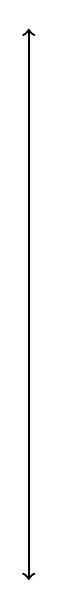
\begin{tikzpicture}
      \draw[<->, thick] (0,1)--(0,8);
      \vspace{1cm}
    \end{tikzpicture}
  }



  % ---------------------- CONNEXIONNISTE ------------------------
  \multirow{3}{*}{\vspace{-13.8cm}\textbf{$\sim$ \textit{Connectionist}}}
  \vspace{-0.35cm}
                           & \textbf{Maintaining simulation/real-world consistency}

  {\tiny \begin{spacing}{0.8}
             \textbf{Robust RL}~\parencite{pinto2017robust}, \textbf{Sim2Real}~\parencite{tobin2017domain,ganin2016domain}, \textbf{dynamic calibration}~\parencite{deisenroth2011pilco}
           \end{spacing}}

                           & {\vspace{-0.12cm}$\sim$~--~\cmark }                               & {\vspace{-0.12cm}n/a }             & {\vspace{-0.12cm} \cmark }          & {\vspace{-0.12cm} $\sim$ }          & {\vspace{-0.12cm} $\sim$ }                                 \\

                           & \textbf{MARL \& organizational constraints}

  {\tiny \begin{spacing}{0.8}
             \textbf{CPO}~\parencite{achiam2017constrained}, \textbf{Deep Constrained Q-Learning}~\parencite{kalweit2020deep}, \textbf{Safe RL}~\parencite{garcia2015comprehensive}, \textbf{Deep TAMER}~\parencite{warnell2018deep}, \textbf{reward shaping}~\parencite{ng1999policy}, \textbf{shielding}~\parencite{amodei2016concrete}
           \end{spacing}}

                           & {\vspace{0.06cm}\xmark~--~$\sim$ }                                & {\vspace{0.06cm}$\sim$~--~\cmark } & {\vspace{0.06cm} $\sim$ }           & {\vspace{0.06cm} \cmark }           & {\vspace{0.06cm} $\sim$~--~\cmark }                        \\

                           & \textbf{Emergent organizational extraction}
  {\tiny \begin{spacing}{0.8}
             \textbf{tree extraction}~\parencite{milani2022maviper,zhang2024advancing}, \textbf{value decompositions}~\parencite{Sunehag2018,Tabish2018}, \textbf{Shapley attributions}~\parencite{heuillet2021collective}, \textbf{emergent role inference}~\parencite{Wang2020}
           \end{spacing}}

                           & {\vspace{0.06cm} \xmark~--~$\sim$ }                               & {\vspace{0.06cm} $\sim$  }         & {\vspace{0.06cm} $\sim$ }           & {\vspace{0.06cm} \xmark~--~$\sim$ } & {\vspace{0.06cm} \cmark }                                  \\[0.001cm]
  \hline
\end{tabular}
